\documentclass[aspectratio=169,10pt]{beamer}
\usepackage{../common/beamer_theme_bio}

\title{\textbf{Biostatistiques Appliquées}}
\subtitle{Chapitre III : Corrélation, Régression Linéaire \& Gammes d'Étalonnage}
\author{\textbf{Dr. Sarra BENMOUMOU (Ph.D.)}}
\institute{
  Faculté des Sciences --- Département de Biologie\\
  Master 2 : Biochimie Appliquée\\
  \textbf{Université M'Hamed Bougara de Boumerdès (UMBB)}
}
\date{Année Universitaire 2024 -- 2025}

\begin{document}

\begin{frame}[plain]
  \titlepage
\end{frame}

\begin{frame}{Plan Détaillé du Chapitre III}
  \tableofcontents
\end{frame}

% ========================================================
\section{Corrélation vs. Régression}
% ========================================================

\begin{frame}{Deux Concepts Complémentaires mais Très Différents}
  \begin{columns}[onlytextwidth, T]
    \begin{column}{0.48\linewidth}
      \begin{conceptbox}{1. La Corrélation ($r$ ou $\rho$)}
        \begin{itemize}
          \item Mesure l'\textbf{intensité et le sens} de l'association entre deux variables.
          \item Rôle strictement \textbf{symétrique} : $\text{cor}(X,Y) = \text{cor}(Y,X)$.
          \item Pas de notion de variable explicative ni de variable réponse.
        \end{itemize}
      \end{conceptbox}
    \end{column}
    \begin{column}{0.48\linewidth}
      \begin{conceptbox}{2. La Régression Linéaire}
        \begin{itemize}
          \item Modélise une relation de \textbf{dépendance fonctionnelle asymétrique} : $Y = f(X)$.
          \item $X$ est la variable contrôlée (ex: concentration connue d'étalon BSA).
          \item $Y$ est la réponse biologique (ex: absorbance $A_{595}$).
          \item Permet la \textbf{prédiction inverse} d'échantillons inconnus.
        \end{itemize}
      \end{conceptbox}
    \end{column}
  \end{columns}
  \vspace{1mm}
  \begin{warnbox}{Le Piège Classique : Corrélation $\neq$ Causalité}
    Une forte corrélation entre deux marqueurs sériques ne prouve en aucun cas que l'un est la cause de l'autre ! Ils peuvent être co-sécrétés sous l'effet d'une même cytokine inflammatoire.
  \end{warnbox}
\end{frame}

\begin{frame}{Pearson vs. Spearman : Lequel Choisir ?}
  \begin{columns}[onlytextwidth, T]
    \begin{column}{0.48\linewidth}
      \textbf{\color{BioNavy}Coefficient de Pearson ($r$)}
      \begin{equation*}
        r = \frac{\sum (X_i - \bar{X})(Y_i - \bar{Y})}{\sqrt{\sum (X_i - \bar{X})^2 \sum (Y_i - \bar{Y})^2}}
      \end{equation*}
      \begin{itemize}
        \item Mesure une relation strictement \textbf{linéaire}.
        \item Exige la normalité bivariée.
        \item Très vulnérable aux points aberrants d'extrême valeur.
      \end{itemize}
    \end{column}
    \begin{column}{0.48\linewidth}
      \textbf{\color{BioTeal}Coefficient de Spearman ($\rho$)}
      \begin{equation*}
        \rho = 1 - \frac{6 \sum d_i^2}{n(n^2 - 1)}
      \end{equation*}
      \begin{itemize}
        \item Mesure une association \textbf{monotone} quelconque (croissance continue même courbée).
        \item Basé sur les \textbf{rangs} relatifs des mesures.
        \item Insensible aux valeurs aberrantes et aux non-normalités.
      \end{itemize}
    \end{column}
  \end{columns}
\end{frame}

% ========================================================
\section{Modèle Linéaire Simple \& Moindres Carrés}
% ========================================================

\begin{frame}{Principe Fondamental des Moindres Carrés Ordinaires (MCO)}
  \begin{conceptbox}{Équation du Modèle Linéaire}
    \begin{equation*}
      Y_i = \beta_0 + \beta_1 X_i + \varepsilon_i \quad \text{avec } \varepsilon_i \sim \mathcal{N}(0, \sigma^2)
    \end{equation*}
  \end{conceptbox}
  \begin{columns}[onlytextwidth, T]
    \begin{column}{0.48\linewidth}
      \textbf{\color{BioNavy}Principe Géométrique :}
      Minimiser la somme des carrés des écarts verticaux (résidus) entre les points observés et la droite :
      \begin{equation*}
        \min \sum_{i=1}^n e_i^2 = \min \sum_{i=1}^n (Y_i - (\hat{\beta}_0 + \hat{\beta}_1 X_i))^2
      \end{equation*}
    \end{column}
    \begin{column}{0.48\linewidth}
      \textbf{\color{BioTeal}Formules des Estimateurs :}
      \begin{align*}
        \hat{\beta}_1 &= \frac{\sum (X_i - \bar{X})(Y_i - \bar{Y})}{\sum (X_i - \bar{X})^2} = \frac{\text{Cov}(X,Y)}{\text{Var}(X)} \\
        \hat{\beta}_0 &= \bar{Y} - \hat{\beta}_1 \bar{X}
      \end{align*}
    \end{column}
  \end{columns}
\end{frame}

% ========================================================
\section{Étude de Cas : Gamme Bradford \& Limites LOD/LOQ}
% ========================================================

\begin{frame}{Gamme Étalon Bradford : Droite \& Bandes de Confiance}
  \begin{center}
    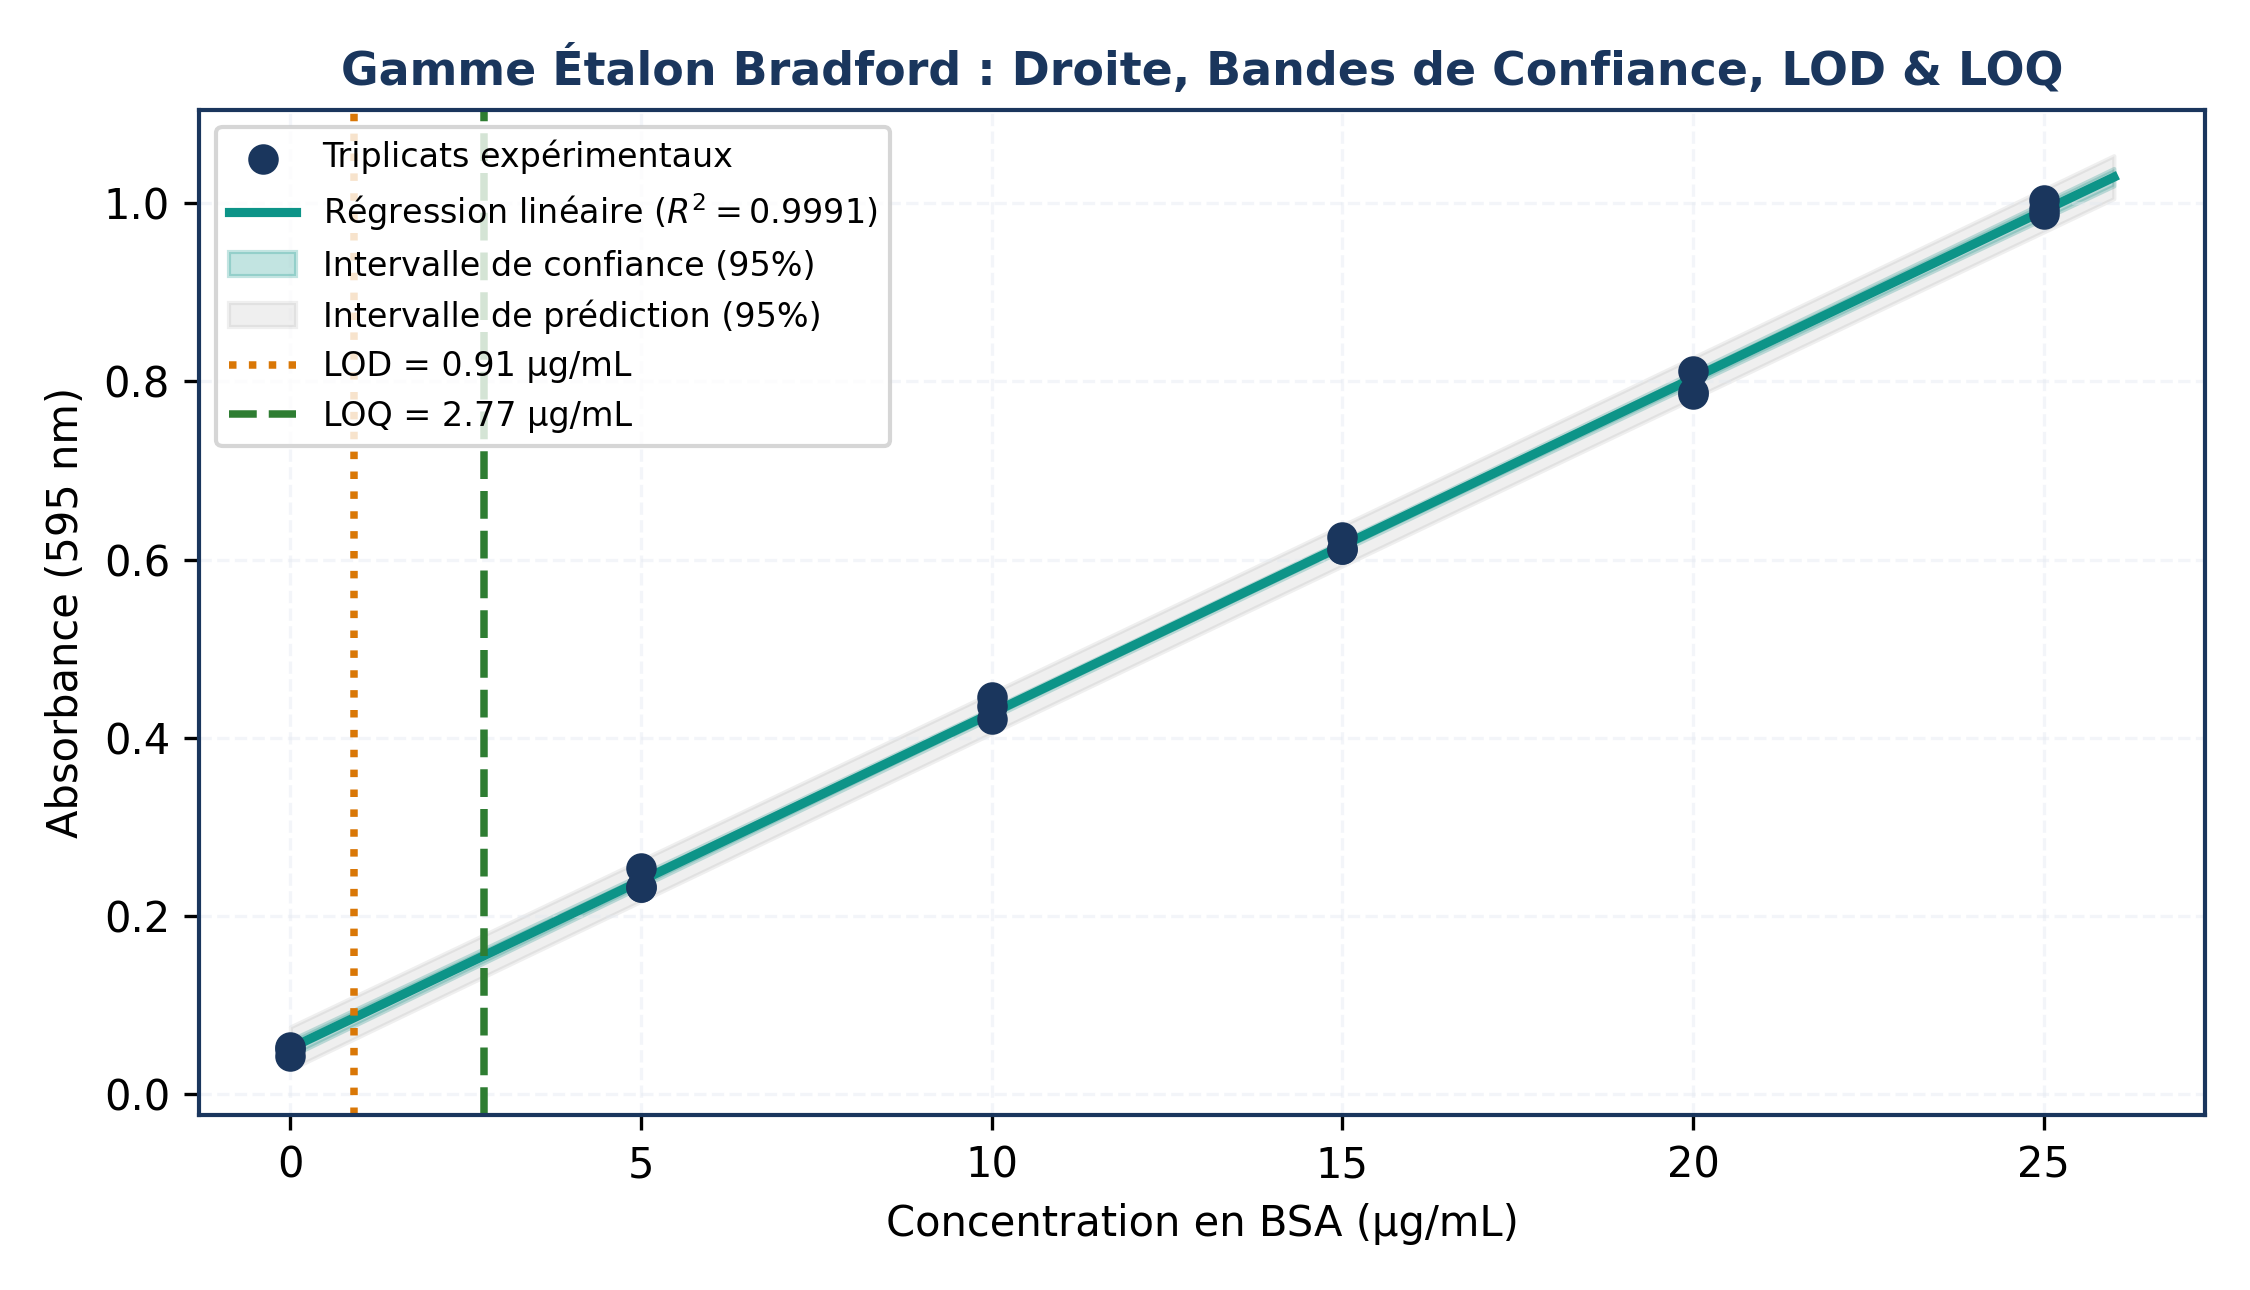
\includegraphics[width=0.88\linewidth]{../figures/fig03_bradford_calibration.png}
  \end{center}
  \vspace{-2mm}
  \begin{columns}[onlytextwidth, T]
    \begin{column}{0.48\linewidth}
      {\footnotesize \textbf{Bande de confiance (95\%) :} Zone où se situe la vraie droite moyenne de calibration.}
    \end{column}
    \begin{column}{0.48\linewidth}
      {\footnotesize \textbf{Bande de prédiction (95\%) :} Zone beaucoup plus large contenant 95\% des mesures individuelles futures.}
    \end{column}
  \end{columns}
\end{frame}

\begin{frame}{Sensibilité Analytique : Limites LOD et LOQ}
  \begin{conceptbox}{Critères Officiels (Recommandations ICH Q2B)}
    À partir de l'écart-type résiduel de la droite $s_{\text{res}}$ et de la pente $\hat{\beta}_1$ (sensibilité) :
    \begin{columns}[onlytextwidth, T]
      \begin{column}{0.48\linewidth}
        \textbf{Limite de Détection (LOD) :}
        Plus petite quantité discernable du blanc :
        \begin{equation*}
          \mathbf{LOD} = \frac{3.3 \cdot s_{\text{res}}}{\hat{\beta}_1} = 0.94\,\mu\text{g/mL}
        \end{equation*}
      \end{column}
      \begin{column}{0.48\linewidth}
        \textbf{Limite de Quantification (LOQ) :}
        Plus petite quantité mesurable avec précision :
        \begin{equation*}
          \mathbf{LOQ} = \frac{10.0 \cdot s_{\text{res}}}{\hat{\beta}_1} = 2.85\,\mu\text{g/mL}
        \end{equation*}
      \end{column}
    \end{columns}
  \end{conceptbox}
  \vspace{1mm}
  \begin{takeawaybox}{Pratique du Dosage d'un Échantillon Inconnu}
    Pour $A_{595} = 0.427$ mesuré sur un extrait tissulaire :
    $$[\text{Protéine}] = \frac{0.427 - 0.045}{0.0382} = \mathbf{10.00\,\mu\text{g/mL}}$$
    Puisque $10.00 > \text{LOQ}$, le résultat est rigoureusement validé et publiable !
  \end{takeawaybox}
\end{frame}

% ========================================================
\section{Diagnostic des Résidus}
% ========================================================

\begin{frame}{Comment Valider l'Ajustement Linéaire ?}
  \begin{center}
    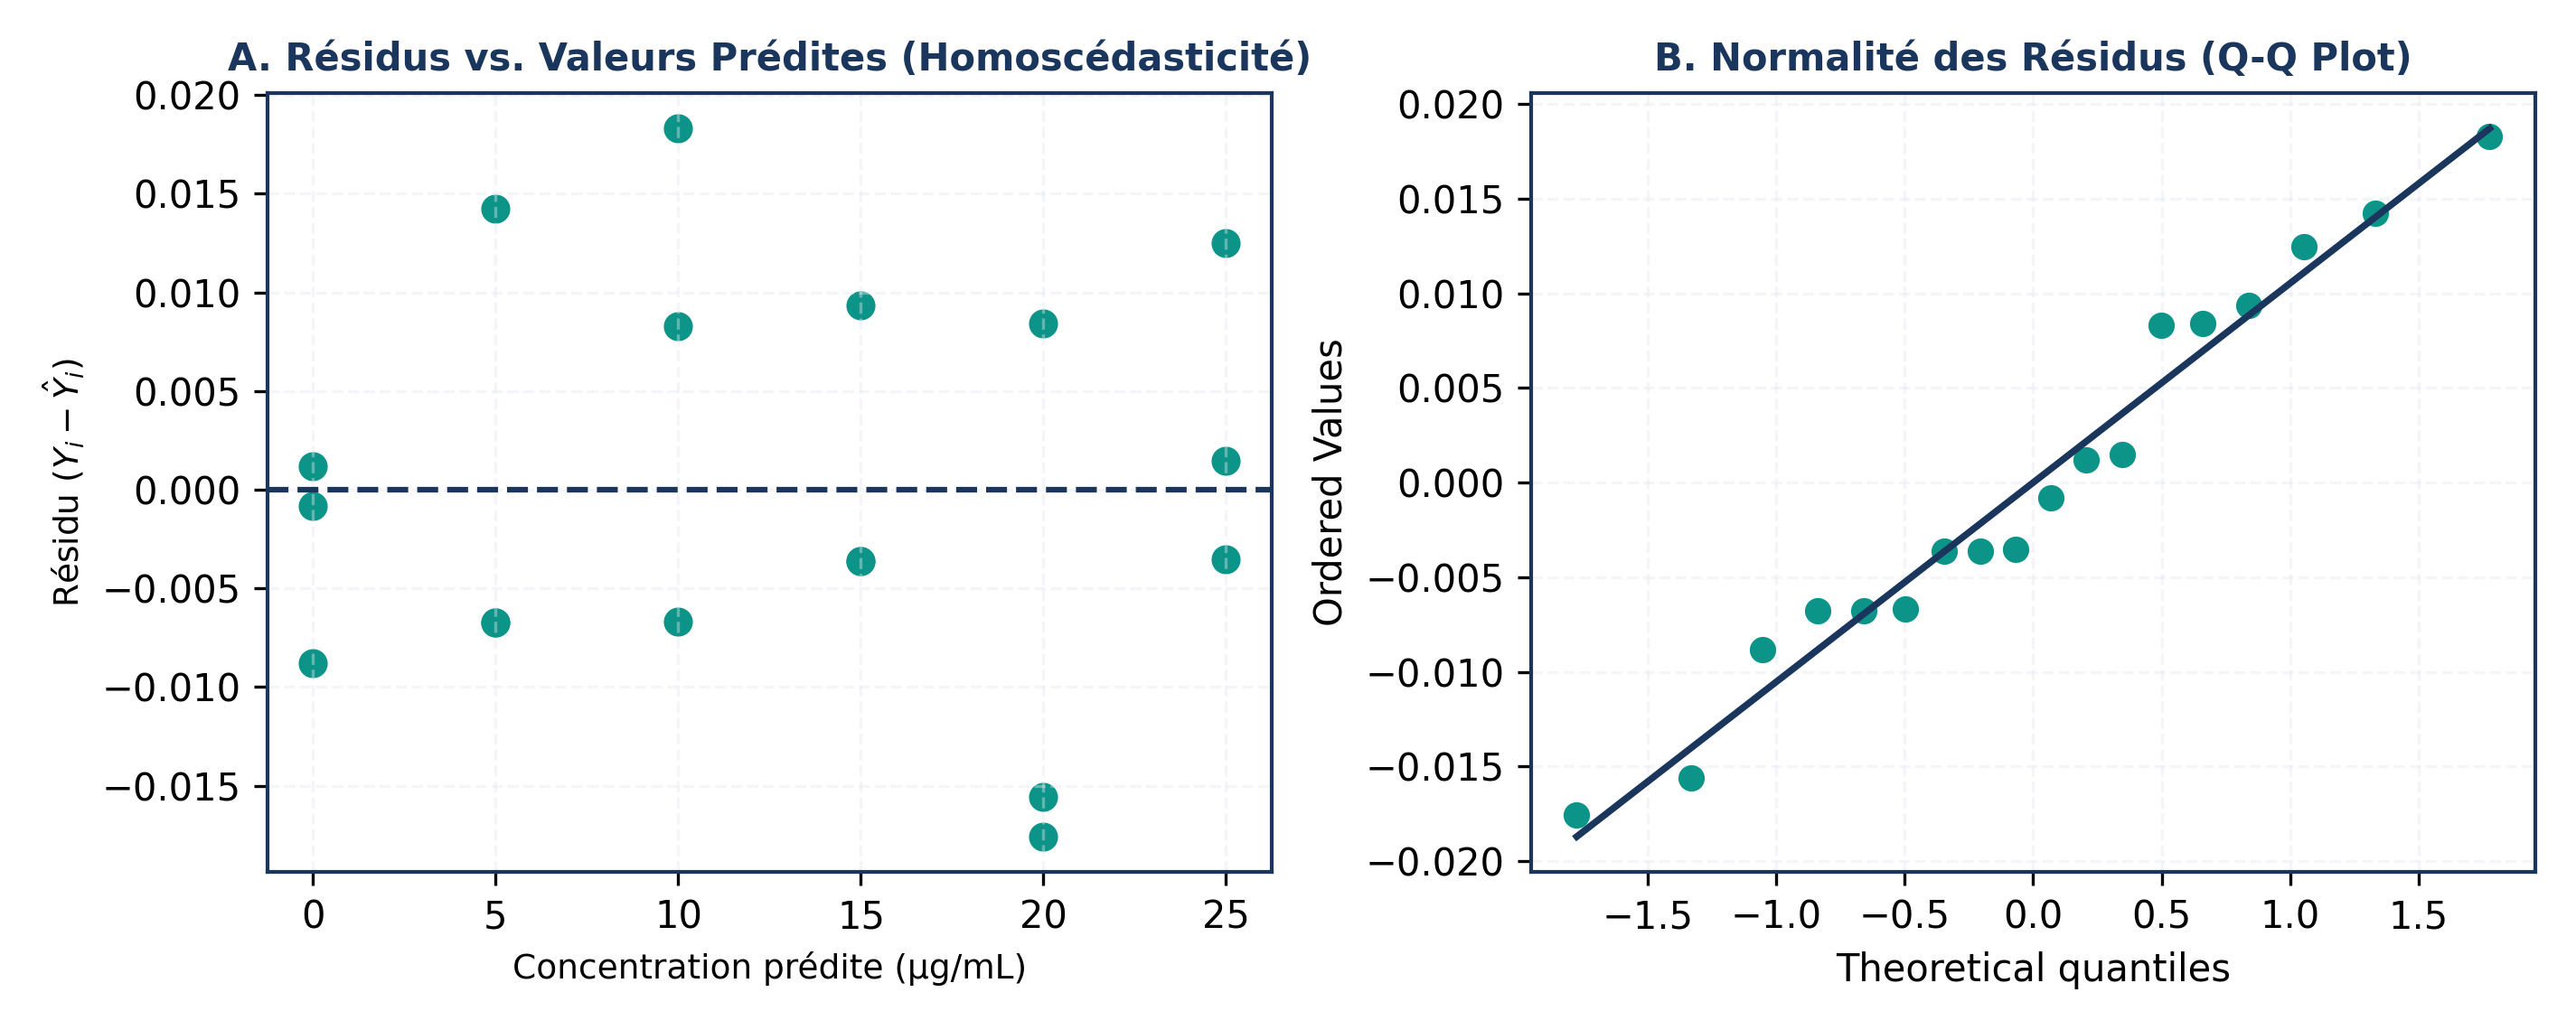
\includegraphics[width=0.90\linewidth]{../figures/fig03_residuals_diagnostics.png}
  \end{center}
  \vspace{-2mm}
  \begin{columns}[onlytextwidth, T]
    \begin{column}{0.48\linewidth}
      {\footnotesize \textbf{À gauche (Homoscédasticité) :} Résidus répartis de manière aléatoire et symétrique autour de zéro. Aucune tendance en courbe ou en entonnoir.}
    \end{column}
    \begin{column}{0.48\linewidth}
      {\footnotesize \textbf{À droite (Normalité) :} Les points suivent la droite quantile-quantile (Q-Q plot), confirmant que les erreurs de pipetage suivent la loi normale.}
    \end{column}
  \end{columns}
\end{frame}

\begin{frame}[plain]
  \begin{center}
    \vspace{1.8cm}
    {\Huge\color{BioNavy}\textbf{Fin du Chapitre III}}\\[0.8cm]
    {\large Prochaine étape : La Régression Non Linéaire en Biochimie}\\[1.2cm]
    \textbf{Dr. Sarra BENMOUMOU (Ph.D.)}\\
    \small Faculté des Sciences --- Département de Biologie\\
    \textbf{Université M'Hamed Bougara de Boumerdès (UMBB)}
  \end{center}
\end{frame}

\end{document}
